\documentclass[a4paper, 12pt]{article}

% Configuration {{{
\usepackage[utf8]{inputenc}
\usepackage[T2A]{fontenc} % T1 for English
\usepackage[english, russian]{babel}

\usepackage{enumitem}
\setlist{nolistsep}
\usepackage{mathtools}
\usepackage{xcolor}
\definecolor{dimblue}{HTML}{1010aa}
\usepackage[
	colorlinks=true, 
	allcolors=dimblue
]{hyperref}
\usepackage[
	vmargin=1in,
	hmargin=1in
]{geometry}
\linespread{1.3}
\usepackage{indentfirst}
\usepackage{graphicx}
\usepackage{tikz}
\usepackage[multidot]{grffile}
\usepackage[labelsep=period]{caption}
\usepackage{subcaption}
\usepackage{multirow}

%\usepackage{times} % for English

\usepackage{colortbl}
\usepackage{pgfplots}
\pgfplotsset{major grid style={dashed,lightgray}}

\def\d{\mathrm{d}}
\def\Li{$^6$}
\def\Ca{$^{40}$}
\def\ompI{J. Cook}
\def\ompII{R. Kalpakchieva \textit{et al.}}
\def\ompIII{R. O. Akyuz, A. Winther}
% }}}

\begin{document}

\begin{center}% Title {{{
	\textbf{\large Упругое рассеяние $^6$Li на ядрах $^{40}$Ca 
	при~энергиях 20, 26, 28, 30, 32, 34, 88, 99, 156, 210, 240 МэВ}

	Керим Гусейнов

	Группа 213М
\end{center}% }}}

% Intro {{{
В данной работе изучается упругое рассеяние ядер $^6$Li на мишени 
$^{40}$Ca при энергиях в лабораторной системе отсчета, равных 
20~\cite{20mev}, 26~\cite{26-28-30-34mev}, 
28~\cite{26-28-30-34mev,28-34mev}, 30~\cite{26-28-30-34mev,30mev}, 
32~\cite{32mev}, 34~\cite{26-28-30-34mev,28-34mev}, 88~\cite{88mev}, 
99~\cite{99mev}, 156~\cite{156mev}, 210~\cite{210mev}, 
240~МэВ~\cite{240mev}. Работа осуществляется с помощью базы знаний 
NRV~\cite{nrv} на основе задач 1 и 2, поставленных 
в пособии~\cite{tutorial}.
% }}}

% Task 1 {{{
\begin{center}
	\textbf{\large Задание 1. Сравнение экспериментальных сечений 
	с~формулой Резерфорда}
\end{center}

Кулоновский потенциал уникален тем, что и при классическом, и при 
квантовом рассмотрении дает один результат для сечения -- формулу 
Резерфорда. При учете движения центра масс и подстановке всех численных 
значений формула Резерфорда приобретает следующий вид:
\begin{equation}\begin{aligned}% Rutherford {{{
	\left(\frac{\d\sigma}{\d\Omega}\left(\theta_{\mathrm{c.m.}}\right)\right)_\text{Ruth.}
	& = \left(\frac{Z_1 Z_2 e^2}{4 E_\text{c.m.}}\right)^2
	\frac{1}{\sin^4\left(\theta/2\right)} \\
	& = \left(\frac{Z_1 Z_2 e^2}{4 \frac{m_2}{m_1 + m_2} E_\text{lab.}}\right)^2
	\frac{1}{\sin^4\left(\theta/2\right)} \\
	& = \left(\frac{3\cdot20 \cdot 197/137}{4 \frac{40}{6 + 40} E_\text{lab.}^\text{MeV}}\right)^2
	\frac{1}{\sin^4\left(\theta/2\right)} \text{ фм}^2/\text{ср} \\
	& = \left(\frac{3\cdot20 \cdot 197/137}{4 \frac{40}{6 + 40} E_\text{lab.}^\text{MeV}}\right)^2
	\frac{1}{\sin^4\left(\theta/2\right)} \cdot 10 \text{ мб/ср} \\
	& = 6152.75 \cdot {(E_\text{lab.}^\text{MeV})^{-2}}
	\frac{1}{\sin^4\left(\theta/2\right)} \text{ мб/ср} \\
	\label{eq:ruth}
\end{aligned}\end{equation}% }}}
При взаимодействии ядерных систем кулоновская компонента потенциала 
оказывается не единственной. Кроме того, учет размеров ядра будет еще 
больше искажать картину. Вследствие этого возникают существенные 
отклонения даже в классическом случае, как будет видно в дальнейшем на 
рисунках~\ref{fig:28mev-abs-ratio}, \ref{fig:30mev-abs-ratio}, 
\ref{fig:99mev-abs-ratio}.

С помощью базы знаний NRV были получены экспериментальные сечения 
рассеяния \Li Li на \Ca Ca при различных энергиях. Они представлены на 
рисунках~\ref{fig:othermev-cmp}, \ref{fig:28mev-cmp}, 
\ref{fig:30mev-cmp}, \ref{fig:34mev-cmp} в сравнении с сечениями, 
вычисленными по формуле Резерфорда~(\ref{eq:ruth}). Кроме того, на 
рисунках~\ref{fig:28mev-cmp}, \ref{fig:30mev-cmp}, \ref{fig:34mev-cmp} 
сравниваются экспериментальные сечения, полученные различными авторами 
при одинаковых энергиях. Как видно, экспериментальные данные хорошо 
согласуются между собой, но либо подчиняются формуле Резерфорда в узкой 
области малых углов (при энергиях до 34 МэВ), либо не подчиняются вообще 
(при энергиях порядка 100 МэВ и выше). Это связано, во-первых, 
с конечными размерами ядер, а во-вторых -- с присутствием потенциала 
ядерного взаимодействия наравне с электромагнитным. Стоит заметить, что 
величина кулоновского барьера для системы \Li Li+\Ca Ca составляет 
9.3~МэВ, а при энергии 30~МэВ ($E_\text{лаб.}=34$~МэВ) минимальное 
расстояние в 10~фм достигается при угле рассеяния 24\textdegree.

Корректность построенных графиков подтверждается полным их совпадением 
с графиками, предоставляемыми системой NRV, на 
рисунках~\ref{fig:28mev-cmp}, \ref{fig:30mev-cmp}, \ref{fig:34mev-cmp}.

\begin{figure}[b]% low MeV comparison {{{
	\centering
	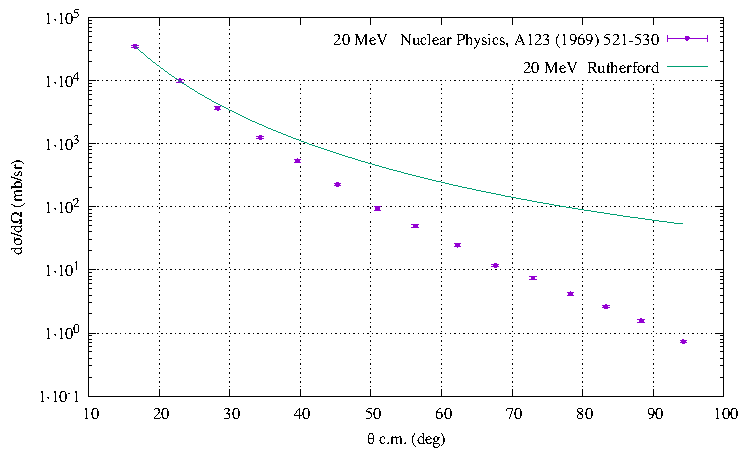
\includegraphics[width=.49\linewidth]{figures/cmp-20mev-abs.pdf}
	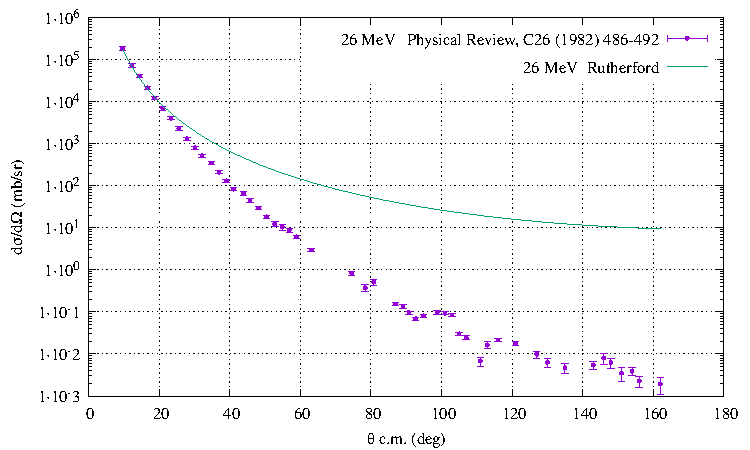
\includegraphics[width=.49\linewidth]{figures/cmp-26mev-abs.pdf}
	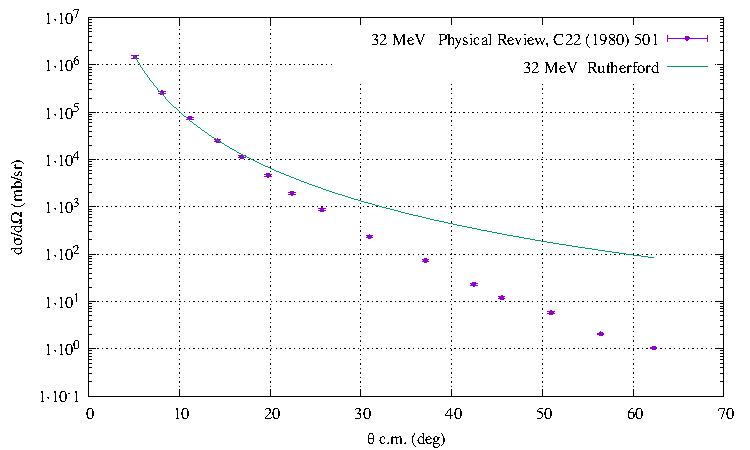
\includegraphics[width=.49\linewidth]{figures/cmp-32mev-abs.pdf}
	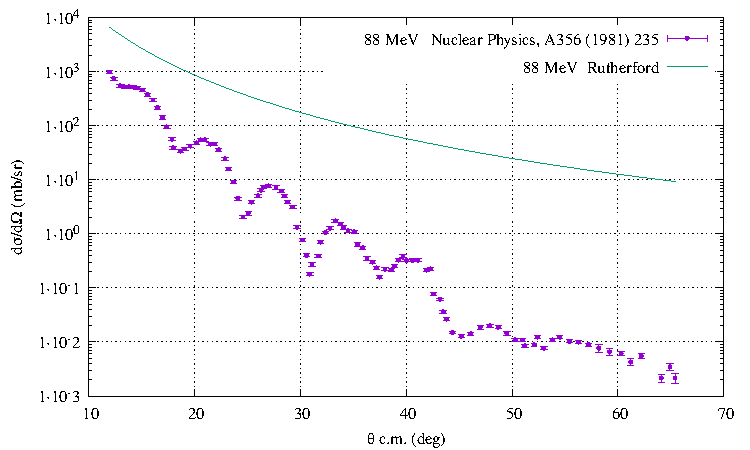
\includegraphics[width=.49\linewidth]{figures/cmp-88mev-abs.pdf}
	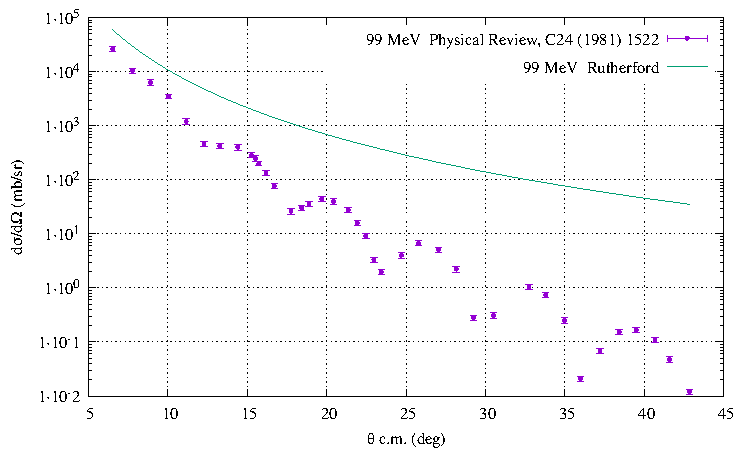
\includegraphics[width=.49\linewidth]{figures/cmp-99mev-abs.pdf}
	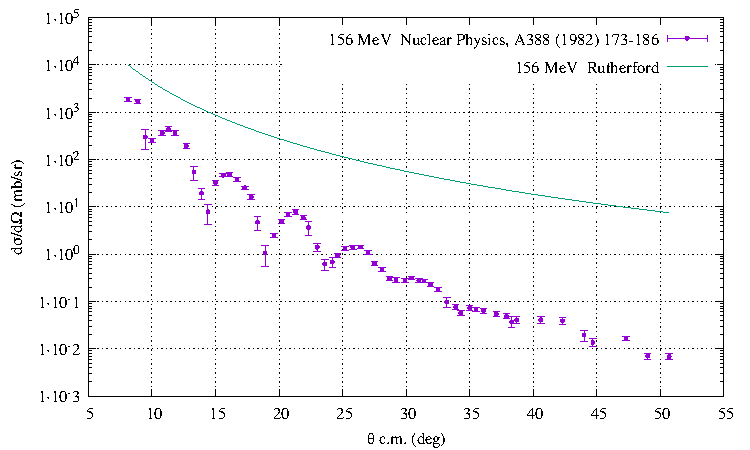
\includegraphics[width=.49\linewidth]{figures/cmp-156mev-abs.pdf}
	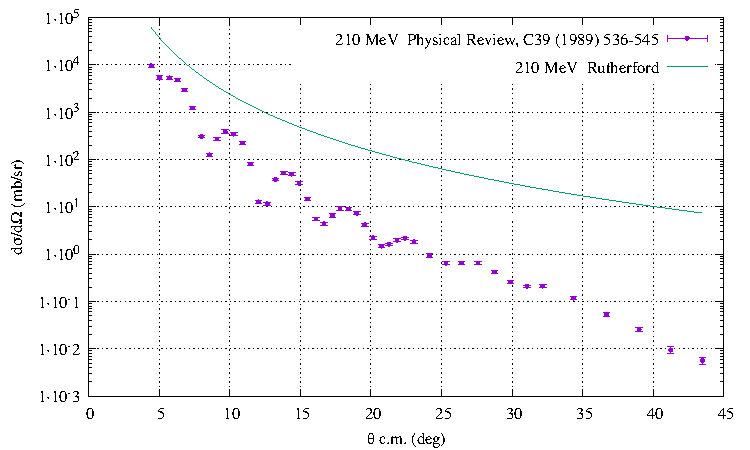
\includegraphics[width=.49\linewidth]{figures/cmp-210mev-abs.pdf}
	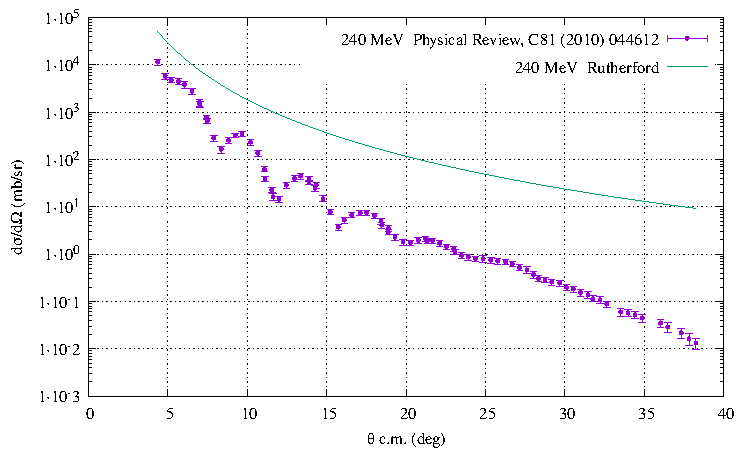
\includegraphics[width=.49\linewidth]{figures/cmp-240mev-abs.pdf}
	\caption{Экспериментальные и Резерфордовские сечения при энергиях от 20 до 240~МэВ.~\cite{20mev,26-28-30-34mev,32mev,88mev,99mev,156mev,210mev,240mev}}
	\label{fig:othermev-cmp}
\end{figure}% }}}

\begin{figure}% 28 MeV comparison {{{
	\centering
	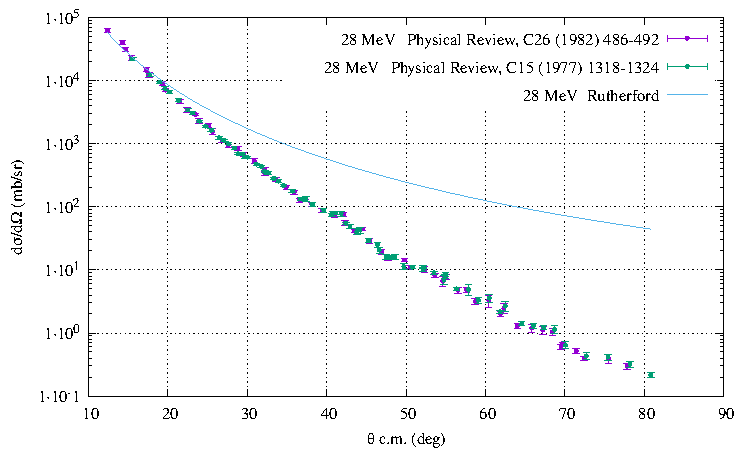
\includegraphics[width=\linewidth]{figures/cmp-28mev-abs.pdf}
	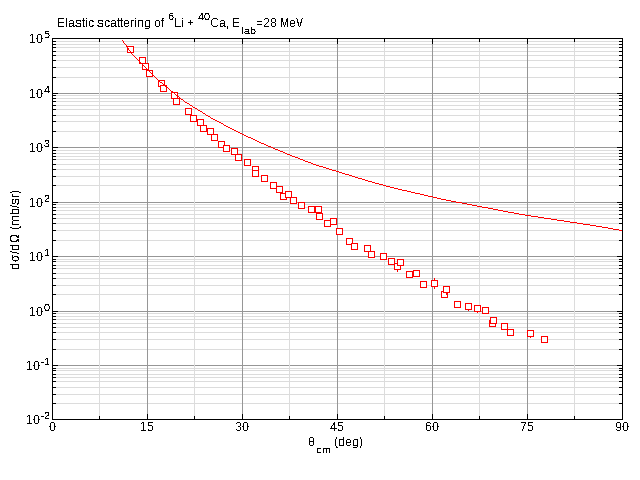
\includegraphics[width=.49\linewidth]{figures/008-28mev-abs.png}
	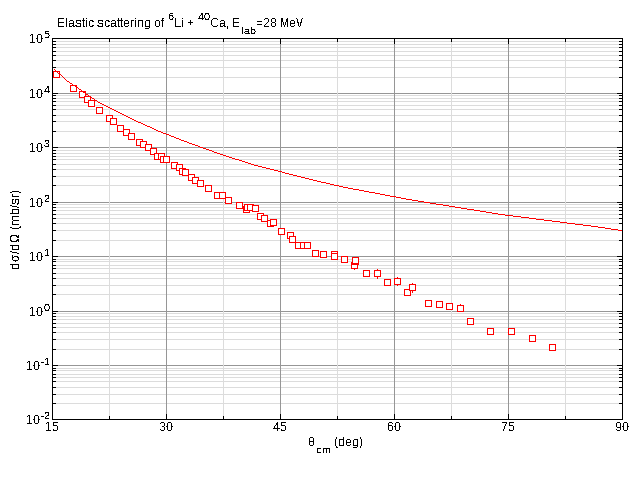
\includegraphics[width=.49\linewidth]{figures/003-28mev-abs.png}
	\parbox{.49\linewidth}{\small\centering Physical Review, C26 (1982) 486-492}
	\parbox{.49\linewidth}{\small\centering Physical Review, C15 (1977) 1318-1324}
	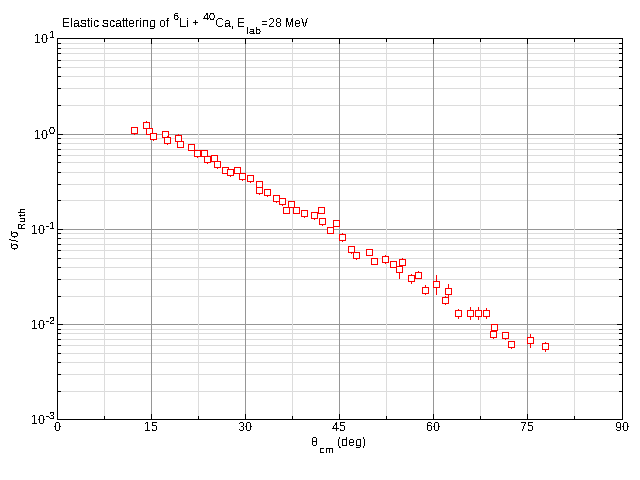
\includegraphics[width=.49\linewidth]{figures/008-28mev-ratio.png}
	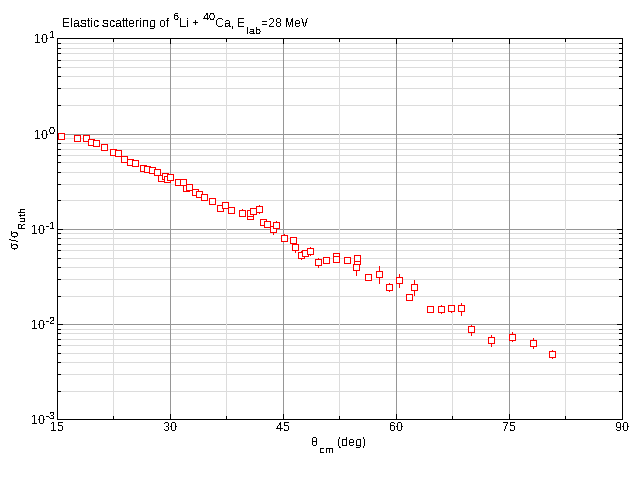
\includegraphics[width=.49\linewidth]{figures/003-28mev-ratio.png}
	\caption{Сравнение сечений, полученных разными авторами при энергии 28~МэВ.~\cite{26-28-30-34mev,28-34mev}}
	\label{fig:28mev-cmp}
\end{figure}% }}}

\begin{figure}% 30 MeV comparison {{{
	\centering
	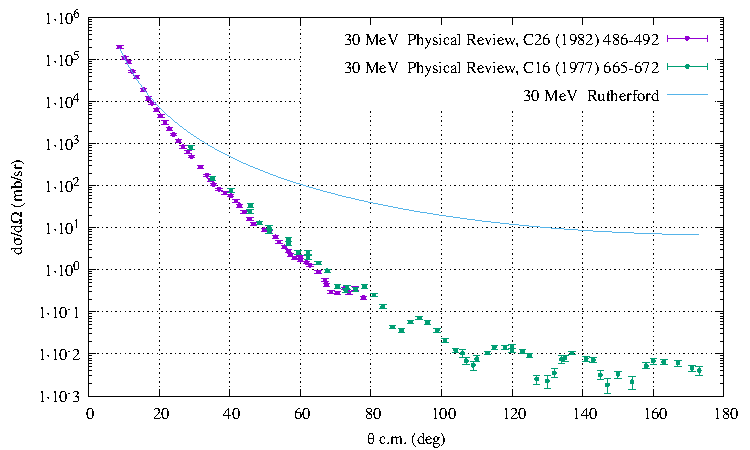
\includegraphics[width=\linewidth]{figures/cmp-30mev-abs.pdf}
	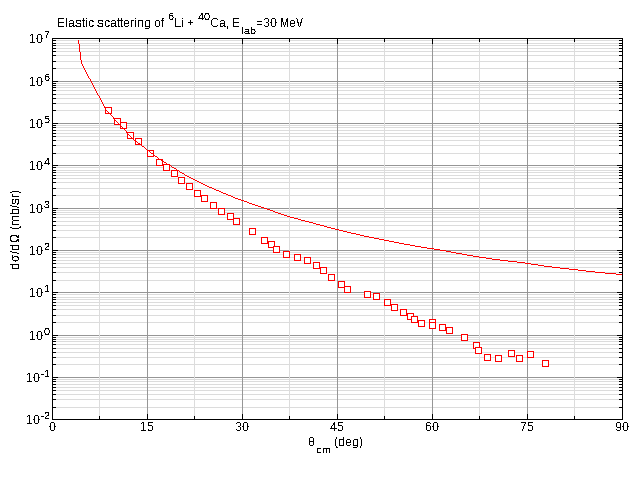
\includegraphics[width=.49\linewidth]{figures/010-30mev-abs.png}
	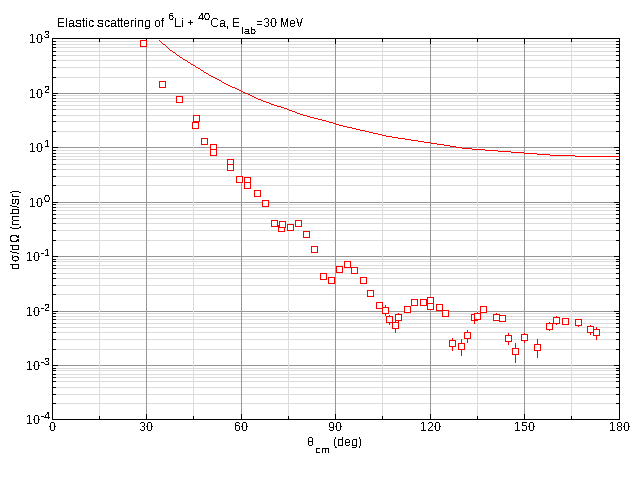
\includegraphics[width=.49\linewidth]{figures/004-30mev-abs.png}
	\parbox{.49\linewidth}{\small\centering Physical Review, C26 (1982) 486-492}
	\parbox{.49\linewidth}{\small\centering Physical Review, C16 (1977) 665-672}
	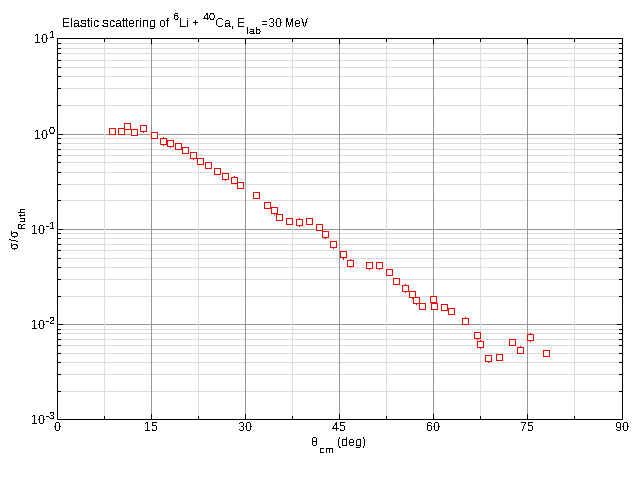
\includegraphics[width=.49\linewidth]{figures/010-30mev-ratio.png}
	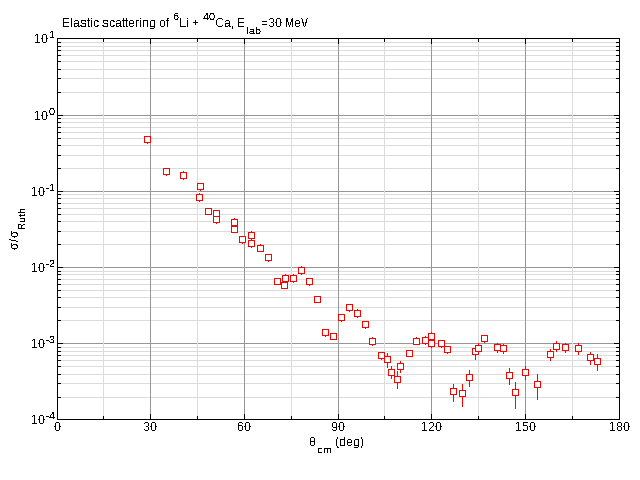
\includegraphics[width=.49\linewidth]{figures/004-30mev-ratio.png}
	\caption{Сравнение сечений, полученных разными авторами при энергии 30~МэВ.~\cite{26-28-30-34mev,30mev}}
	\label{fig:30mev-cmp}
\end{figure}% }}}

\begin{figure}% 34 MeV comparison {{{
	\centering
	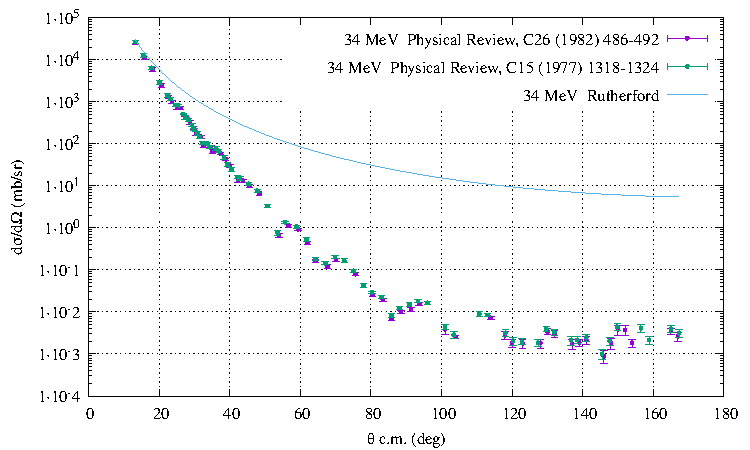
\includegraphics[width=\linewidth]{figures/cmp-34mev-abs.pdf}
	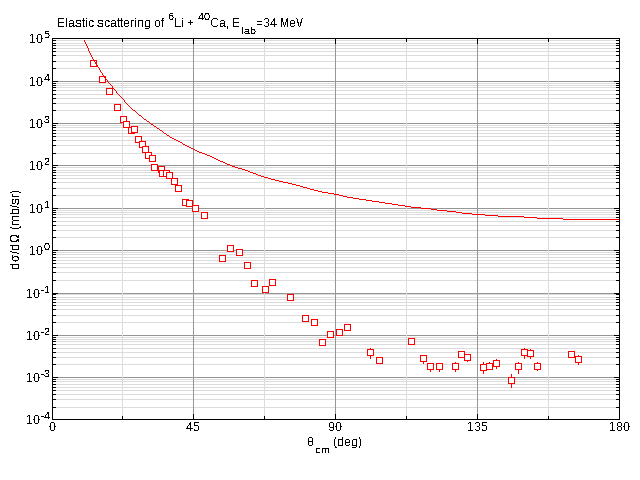
\includegraphics[width=.49\linewidth]{figures/009-34mev-abs.png}
	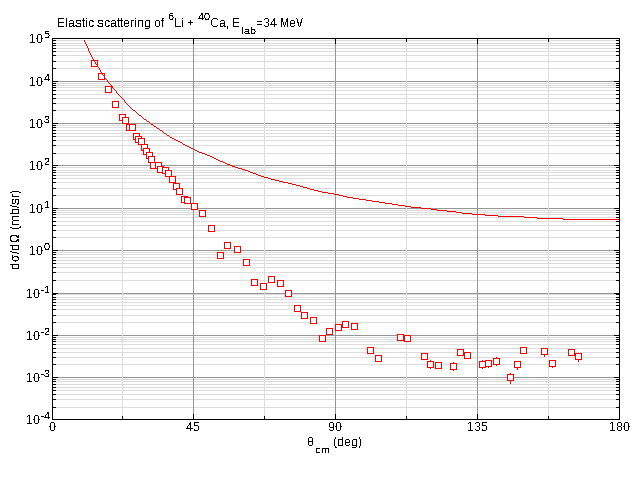
\includegraphics[width=.49\linewidth]{figures/002-34mev-abs.png}
	\parbox{.49\linewidth}{\small\centering Physical Review, C26 (1982) 486-492}
	\parbox{.49\linewidth}{\small\centering Physical Review, C15 (1977) 1318-1324}
	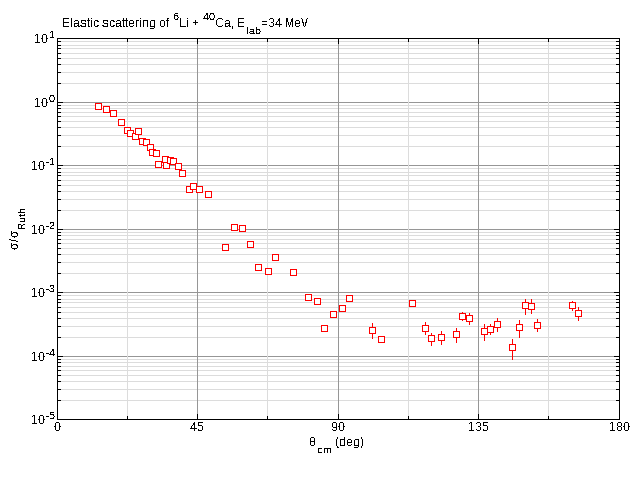
\includegraphics[width=.49\linewidth]{figures/009-34mev-ratio.png}
	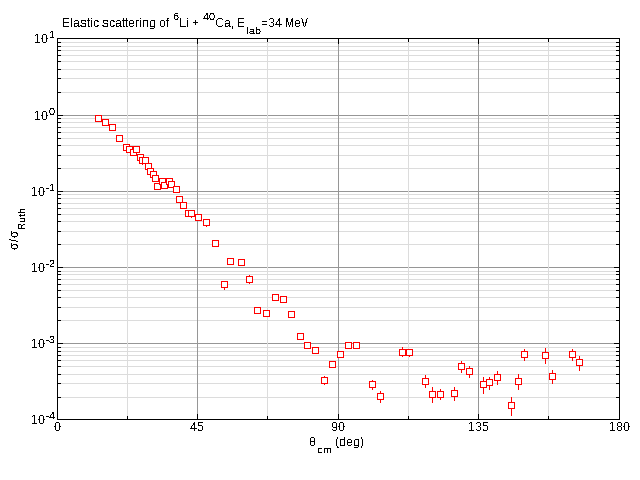
\includegraphics[width=.49\linewidth]{figures/002-34mev-ratio.png}
	\caption{Сравнение сечений, полученных разными авторами при энергии 34~МэВ.~\cite{26-28-30-34mev,28-34mev}}
	\label{fig:34mev-cmp}
\end{figure}% }}}
% }}}

% Task 2 {{{
\clearpage
\begin{center}
	\textbf{\large Задание 2. Рассеяние согласно оптической модели}
\end{center}

Приблизиться к теоретически верному описанию процессов рассеяния ядер 
позволяет оптический потенциал. Путем подбора форм компонент потенциала 
и введения мнимой части появляется возможность более тонко описывать 
взаимодействие ядер и учитывать неупругие каналы.

Система NRV предоставляет возможность выбора различных систематик 
оптического потенциала в случае, когда налетающей частицей является \Li 
Li~\cite{omp1, omp2, omp3}, и аппроксимации экспериментального сечения 
для определения параметров потенциала, с помощью которых затем 
вычисляются волновая функция и $S$\nobreakdash-матрица, а также 
характеристики классического рассеяния.

Для демонстрации процесса выбора наилучшей систематики удобно 
рассмотреть данные для энергии 99~МэВ~\cite{99mev}, поскольку это 
наивысшая доступная энергия, на которую еще рассчитаны все три 
систематики. Для каждой систематики производилась аппроксимация при 
последовательном варьировании различных параметров, включая ширины 
диффузных слоев вещественной и мнимой частей потенциала, до тех пор, 
пока значение $\chi^2/N_\text{точек}$ не переставало уменьшаться. 
Полученные в итоге параметры потенциалов, а также сечение поглощения 
и полное сечение рассеяния, выписаны в таблице~\ref{tab:99mev-omp123}. 
Сами потенциалы и дифференциальные сечения рассеяния показаны на 
рисунке~\ref{fig:99mev-omp123}. Как видно, наилучшая аппроксимация 
достигается при выборе систематики \ompIII, однако в этом случае 
потенциал в центре отталкивающий, а не притягивающий, какой следует 
ожидать от ядерного взаимодействия. Поэтому для дальнейшего анализа 
набора данных при 99~МэВ была выбрана систематика \ompI. Стоит обратить 
внимание, что для разных энергий наилучшее описание достигалось при 
использовании разных систематик. Кроме того, для энергий 156, 210 
и 240~МэВ была доступна лишь систематика \ompIII.

\begin{table}[b]% omp123, 99mev {{{
	\caption{Сравнение параметров оптической модели, сечений поглощения и полных сечений для разных систематик при аппроксимации экспериментального сечения при энергии 99~МэВ.~\cite{99mev}}
	\label{tab:99mev-omp123}
	\centering\scriptsize
	\begin{tabular}{c|ccc|ccc}
		\multirow{2}{*}{OMP систематика} & \multicolumn{3}{c|}{Вещественная часть} &
		\multicolumn{3}{c}{Мнимая часть} \\
		 & $V_0$, МэВ & $r_0(R)$, фм & $a$, фм & $V_0$, МэВ & $r_0(R)$, фм & $a$, фм \\
		 \hline
		J. Cook~\cite{omp1} & --117.158 & 0.881 (4.614) & 0.769 & --22.871 & 1.155 (6.049) & 0.874 \\
		R. Kalpakchieva \textit{et al.}~\cite{omp2} & --137.088 & 0.828 (4.336) & 0.813 & --20.906 & 1.187 (6.216) & 0.826 \\
		R. O. Akyuz, A. Winther~\cite{omp3} & --7.321 & 1.372 (7.185) & 0.728 & --71.512 & 1.044 (5.468) & 0.692 \\
		\hline
	\end{tabular}
	\vskip-.1\baselineskip
	\begin{tabular}{c|ccc}
		OMP систематика & $\sigma_\text{R}$, мб & $\sigma_\text{tot}$, мб & $\chi^2/N$ \\
		 \hline
		J. Cook~\cite{omp1} & 2048.19 & 3568.68 & 1.496 \\
		R. Kalpakchieva \textit{et al.}~\cite{omp2} & 2009.29 & 3526.60 & 1.601 \\
		R. O. Akyuz, A. Winther~\cite{omp3} & 1859.01 & 3297.10 & 1.290 \\
	\end{tabular}
\end{table}% }}}
\begin{figure}% omp123, 99mev {{{
	\centering
	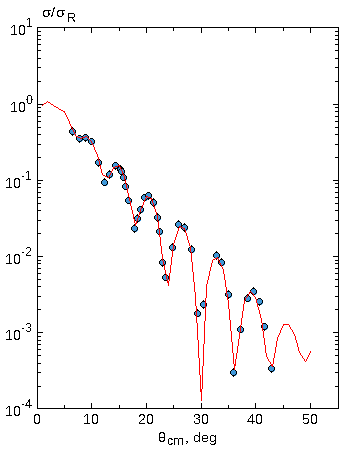
\includegraphics[width=.32\linewidth]{figures/014-omp1-ratio.png}
	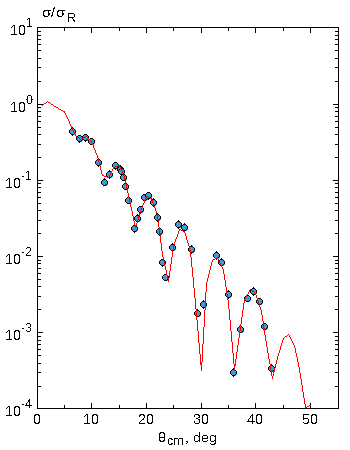
\includegraphics[width=.32\linewidth]{figures/014-omp2-ratio.png}
	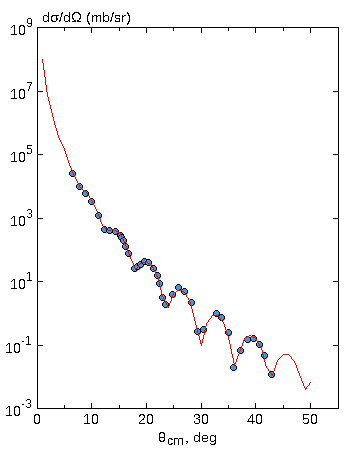
\includegraphics[width=.32\linewidth]{figures/014-omp3-ratio.png}
	\parbox{.32\linewidth}{\centering\footnotesize \ompI}
	\parbox{.32\linewidth}{\centering\footnotesize \ompII}
	\parbox{.32\linewidth}{\centering\footnotesize \ompIII}
	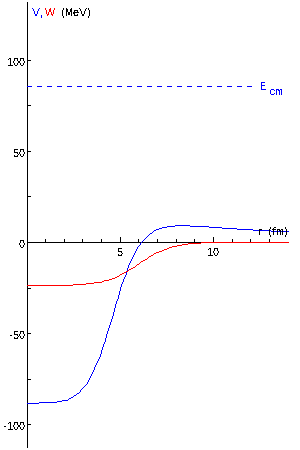
\includegraphics[width=.32\linewidth]{figures/014-omp1-vw.png}
	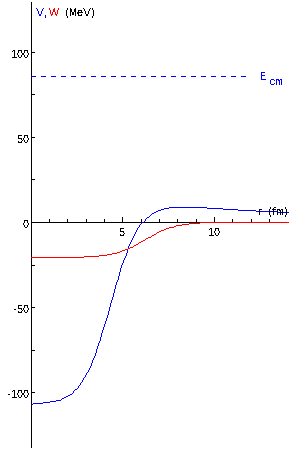
\includegraphics[width=.32\linewidth]{figures/014-omp2-vw.png}
	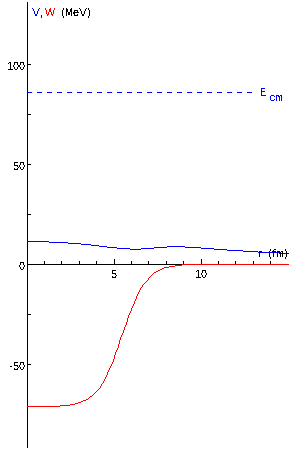
\includegraphics[width=.32\linewidth]{figures/014-omp3-vw.png}
	\caption{Сечения в отношении к Резерфордовскому, вычисленные на основе оптических потенциалов с тремя доступными систематиками, и сами оптические потенциалы. Аппроксимация основана на данных при $E_\text{лаб.} = 99$~МэВ.~\cite{99mev}}
	\label{fig:99mev-omp123}
\end{figure}% }}}

Аналогичным образом были проанализированы все доступные наборы данных, 
а результаты помещены в таблицу~\ref{tab:params}. Полученные потенциалы 
использовались для определения величины и положения кулоновского 
барьера, которые можно найти в таблице~\ref{tab:coul} и на 
рисунке~\ref{fig:coul}. Наблюдается легкая тенденция уменьшения величины 
барьера при увеличении энергии, однако, скорее всего, это лишь видимый 
эффект ввиду недостатка статистики и точности.

\begin{table}% params for E=... {{{
	\caption{Сравнение параметров оптической модели, сечений поглощения и полных сечений при разных энергиях.}
	\label{tab:params}
	\centering\scriptsize
	\begin{tabular}{c|ccc|ccc|ccc}
		\multirow{2}{*}{$E_\text{лаб.}$,~МэВ} & \multicolumn{3}{c|}{Вещественная часть} &
		\multicolumn{3}{c|}{Мнимая часть} & \multirow{2}{*}{$\sigma_\text{R}$, мб} &
		\multirow{2}{*}{$\sigma_\text{tot}$, мб} & \multirow{2}{*}{$\chi^2/N$} \\
		 & $V_0$, МэВ & $r_0(R)$, фм & $a$, фм & $V_0$, МэВ & $r_0(R)$, фм & $a$, фм \\
		 \hline
		20~\cite{20mev} & --108.59 & 0.866 (4.535) & 0.811 & --46.112 & 1.001 (5.242) & 0.884 & 1346.04 & 2179.83 & 6.896 \\
		26~\cite{26-28-30-34mev} & --32.226 & 1.261 (6.604) & 0.591 & --9.339 & 1.239 (6.489) & 0.591 & 1365.94 & 2487.52 & 5.590 \\
		28~\cite{28-34mev} & --316.489 & 0.704 (3.687) & 0.811 & --68.226 & 0.938 (4.912) & 0.884 & 1662.74 & 2790.88 & 2.496 \\
		\arrayrulecolor{lightgray}\hline\arrayrulecolor{black}
		28~\cite{26-28-30-34mev} & --179.076 & 0.793 (4.153) & 0.811 & --69.185 & 0.932 (4.881) & 0.884 & 1656.14 & 2781.48 & 1.818 \\
		30~\cite{30mev} & --37.04 & 1.187 (6.216) & 0.591 & --9.093 & 1.218 (6.379) & 0.591 & 1346.66 & 2456.06 & 16.124 \\
		30~\cite{26-28-30-34mev} & --40.981 & 1.057 (5.536) & 0.811 & --7.484 & 1.355 (7.096) & 0.67 & 1548.24 & 2738.05 & 0.785 \\
		\arrayrulecolor{lightgray}\hline\arrayrulecolor{black}
		32~\cite{32mev} & --31.242 & 1.255 (6.573) & 0.591 & --8.557 & 1.262 (6.609) & 0.591 & 1488.40 & 2754.62 & 3.619 \\
		34~\cite{28-34mev} & --185.6 & 0.805 (4.216) & 0.811 & --10.934 & 1.289 (6.751) & 0.88 & 1863.74 & 3181.27 & 9.658 \\
		34~\cite{26-28-30-34mev} & --55.958 & 1.015 (5.316) & 0.807 & --9.29 & 1.3 (6.808) & 0.714 & 1627.75 & 2900.63 & 9.534 \\
		\arrayrulecolor{lightgray}\hline\arrayrulecolor{black}
		88~\cite{88mev} & --117.84 & 0.876 (4.588) & 0.811 & --20.27 & 1.184 (6.201) & 0.88 & 2081.79 & 3647.99 & 31.544 \\
		99~\cite{99mev} & --117.158 & 0.881 (4.614) & 0.769 & --22.871 & 1.155 (6.049) & 0.874 & 2048.19 & 3568.68 & 1.496 \\
		156~\cite{156mev} & --100.455 & 0.903 (4.729) & 0.795 & --50.918 & 0.98 (5.132) & 0.921 & 2028.83 & 3565.10 & 4.666 \\
		\arrayrulecolor{lightgray}\hline\arrayrulecolor{black}
		210~\cite{210mev} & --9.852 & 1.392 (7.29) & 0.591 & --41.453 & 1.155 (6.049) & 0.583 & 1752.05 & 3221.32 & 23.258 \\
		240~\cite{240mev} & --11.012 & 1.378 (7.217) & 0.591 & --3.448 & 1.328 (6.955) & 0.251 & 983.41 & 3347.94 & 6.212 \\
	\end{tabular}
\end{table}% }}}
\begin{table}% V-coul for E=... {{{
	\caption{Величина и положение кулоновского барьера в оптической модели при различных энергиях столкновения $^6$Li и $^{40}$Ca.}
	\label{tab:coul}
	\centering\scriptsize
	\begin{tabular}{c|cc}
		$E_\text{лаб.}$,~МэВ & $V_\text{кул.}$,~МэВ & $R_\text{кул.}$,~фм \\
		\hline
		20~\cite{20mev} & 9.38 & 8.28 \\
		26~\cite{26-28-30-34mev} & 9.05 & 8.85 \\
		28~\cite{28-34mev} & 9.34 & 8.28 \\
		\arrayrulecolor{lightgray}\hline\arrayrulecolor{black}
		28~\cite{26-28-30-34mev} & 9.34 & 8.28 \\
		30~\cite{30mev} & 9.40 & 8.55 \\
		30~\cite{26-28-30-34mev} & 9.13 & 8.55 \\
		\arrayrulecolor{lightgray}\hline\arrayrulecolor{black}
		32~\cite{32mev} & 9.11 & 8.85 \\
	\end{tabular}
	\begin{tabular}{c|cc}
		$E_\text{лаб.}$,~МэВ & $V_\text{кул.}$,~МэВ & $R_\text{кул.}$,~фм \\
		\hline
		34~\cite{28-34mev} & 9.22 & 8.55 \\
		34~\cite{26-28-30-34mev} & 9.11 & 8.55 \\
		88~\cite{88mev} & 9.22 & 8.82 \\
		\arrayrulecolor{lightgray}\hline\arrayrulecolor{black}
		99~\cite{99mev} & 9.45 & 8.26 \\
		156~\cite{156mev} & 9.29 & 8.24 \\
		210~\cite{210mev} & 9.10 & 8.85 \\
		\arrayrulecolor{lightgray}\hline\arrayrulecolor{black}
		240~\cite{240mev} & 9.10 & 8.85 \\
	\end{tabular}
\end{table}% }}}
\begin{figure}% V-coul vs E {{{
	\centering\small
	\begin{tikzpicture}% {{{
		\begin{axis}[
				x label style={at={(axis description cs:0.87,0)},anchor=north},
				y label style={at={(axis description cs:0,.84)}},
				xmin = 0,
				xlabel={$E_\text{лаб.}$, МэВ},
				ylabel={$V_\text{кул.}$, МэВ},
				grid=both
			]
			\addplot [only marks] table {
				26 9.05
				30 9.13
				32 9.11
				34 9.11
				156 9.29
				240 9.10
				20 9.38
				28 9.34
				28 9.34
				99 9.45
				34 9.22
			};
			\addplot [only marks, color=red] table {
				30 9.40
				88 9.22
				210 9.10
			};
		\end{axis}
	\end{tikzpicture}% }}}
	\caption{Величина кулоновского барьера в оптической модели при столкновении \Li Li и \Ca Ca при энергиях от 20 до 240~МэВ. Красным цветом выделены данные с плохой аппроксимацией.}
	\label{fig:coul}
\end{figure}% }}}

Для трех наборов данных, аппроксимация которых оказалось особенно 
успешной, $E_\text{лаб.}=$ 28~\cite{26-28-30-34mev}, 
30~\cite{26-28-30-34mev}, 99~МэВ~\cite{99mev}, были построены 
парциальные волновые функции и проведено сравнение с классическим 
подходом. Во всех трех случаях из рисунков~\ref{fig:28mev-pdf-traj}, 
\ref{fig:30mev-pdf-traj}, \ref{fig:99mev-pdf-traj} видно, что парциальные 
волновые функции ведут себя одинаково с поправкой на увеличение 
$L_\text{max}$ при большей энергии. А именно, мнимые части волновых 
функций убывают при увеличении орбитального момента, а вещественные 
части вытесняются из области малых расстояний. Это объясняется влиянием 
центробежного барьера, не позволяющего ядрам проникать друг в друга при 
больших орбитальных моментах. Также на 
рисунках~\ref{fig:28mev-pdf-traj}, \ref{fig:30mev-pdf-traj}, 
\ref{fig:99mev-pdf-traj} показаны функция распределения вероятности 
и классические траектории. Можно заметить, что при малых энергиях ядро 
\Li Li в классическом случае может совершить полный оборот вокруг \Ca 
Ca. При энергии 99~МэВ такое поведение не наблюдается, но в функции 
распределения все равно заметны флуктуации при углах рассеяния порядка 
30\textdegree. Аналогичные флуктуации, представляющие собой радужное 
рассеяние, более заметно проявляются при меньших энергиях для гораздо 
большего диапазона углов.

Кроме того, представляет интерес выход из упругого канала, описываемый 
\linebreak $S$\nobreakdash-матрицей в квантовом случае и вероятностью 
поглощения в классическом. Эти величины представлены на 
рисунках~\ref{fig:28mev-abs-ratio}, \ref{fig:30mev-abs-ratio}, 
\ref{fig:99mev-abs-ratio}. Как видно, для 28 и 30~МэВ $\left|S_L\right|$ 
выходит на единицу уже для $L\sim25$, а при 99~МэВ -- только для 
$L\sim70$. Отношение энергий и отношение $L_\text{max}$ совпадают не 
идеально, но весьма близки. Классическая вероятность отсутствия 
поглощения хорошо согласуется с $\left|S_L\right|$ в области, где 
вероятность уже близка к единице. Величина области, в которой поглощение 
практически полное, примерно одинакова для трех энергий и составляет 
5.1~фм.

Классическое и квантовое описания дифференциального сечения также 
представлены на рисунках~\ref{fig:28mev-abs-ratio}, 
\ref{fig:30mev-abs-ratio}, \ref{fig:99mev-abs-ratio}. Очевидно, 
квантовое описание очень хорошо согласуется с данными, поскольку именно 
по этому критерию три набора данных и были отобраны. Классическая кривая 
разумно близка к точкам лишь при углах меньше 30\textdegree{} для 28 
и 30~МэВ и при углах меньше 10{\textdegree} для 99~МэВ. Такое плохое 
описание связано с малостью величины кулоновского барьера.

\begin{figure}% pdf, traj, 28mev {{{
	\centering
	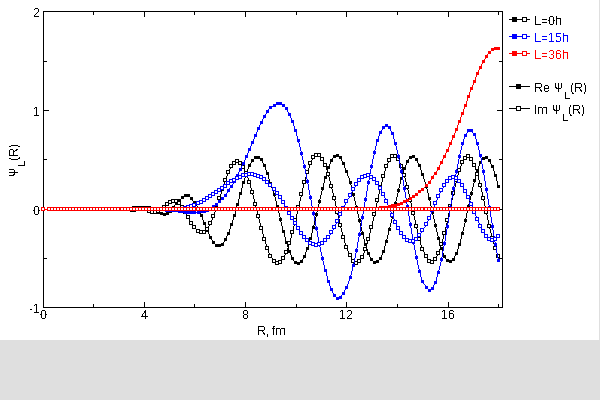
\includegraphics[width=.49\linewidth]{figures/008-omp1-psi.png}
	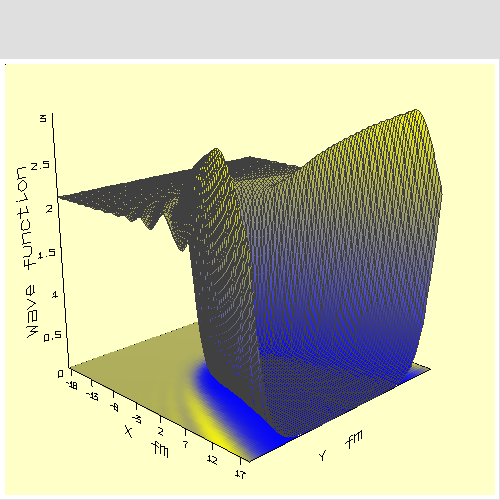
\includegraphics[width=.49\linewidth]{figures/008-omp1-pdf.png}
	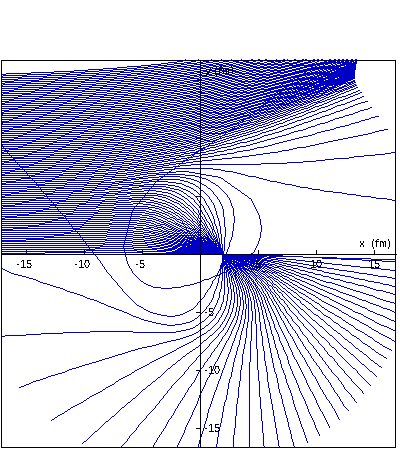
\includegraphics[width=.49\linewidth]{figures/008-clas-traj.png}
	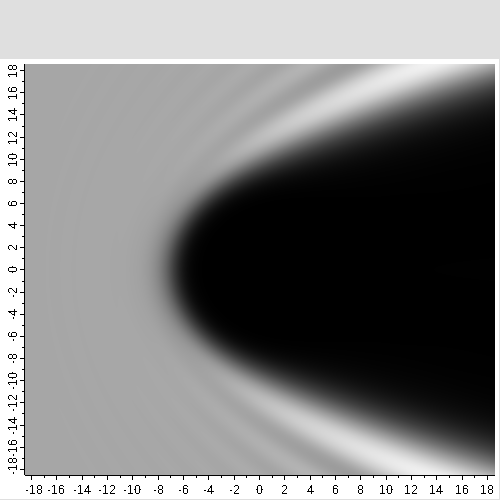
\includegraphics[width=.49\linewidth]{figures/008-omp1-bwpdf.png}
	\caption{Сравнение функции распределения и классических траекторий при энергии 28 МэВ.~\cite{26-28-30-34mev}}
	\label{fig:28mev-pdf-traj}
\end{figure}% }}}
\begin{figure}% abs, ratio, 28mev {{{
	\centering
	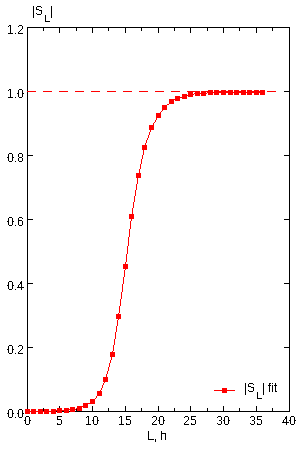
\includegraphics[width=.35\linewidth]{figures/008-omp1-s.png}
	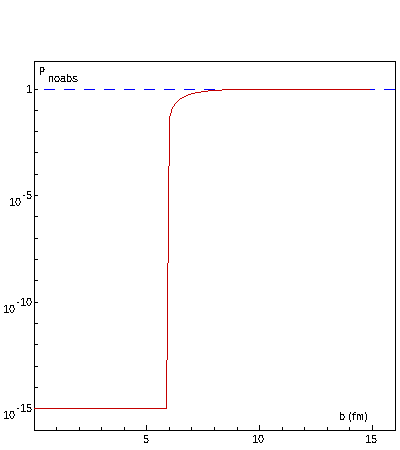
\includegraphics[width=.49\linewidth]{figures/008-clas-surv.png}
	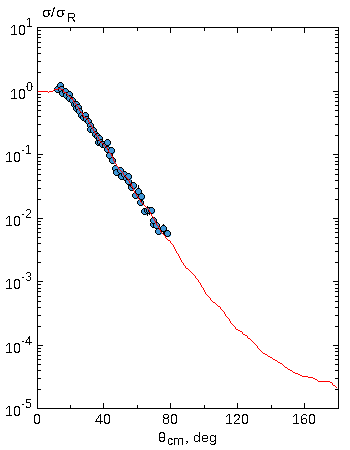
\includegraphics[width=.49\linewidth]{figures/008-omp1-ratio.png}
	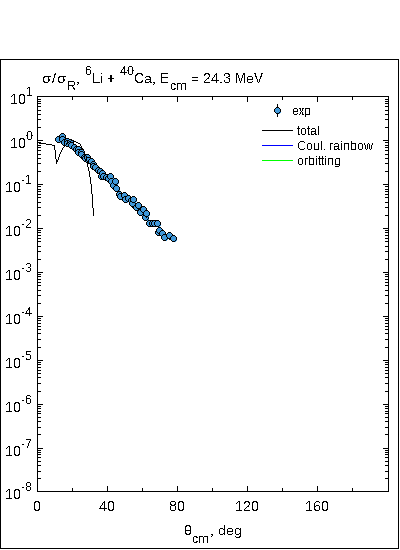
\includegraphics[width=.49\linewidth]{figures/008-clas-ratio.png}
	\caption{Сравнение квантовых и классических вероятностей поглощения и сечений при энергии 28 МэВ.~\cite{26-28-30-34mev}}
	\label{fig:28mev-abs-ratio}
\end{figure}% }}}

\begin{figure}% pdf, traj, 30mev {{{
	\centering
	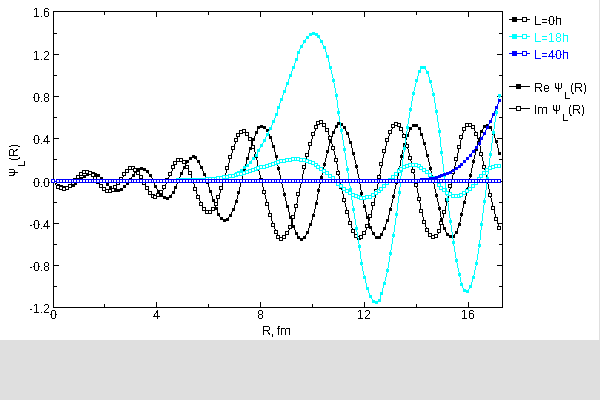
\includegraphics[width=.49\linewidth]{figures/010-omp3-psi.png}
	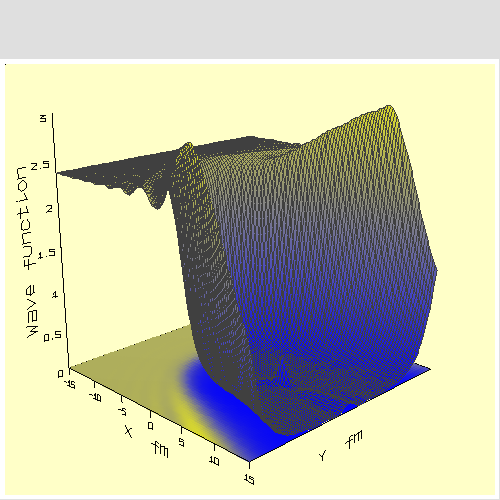
\includegraphics[width=.49\linewidth]{figures/010-omp3-pdf.png}
	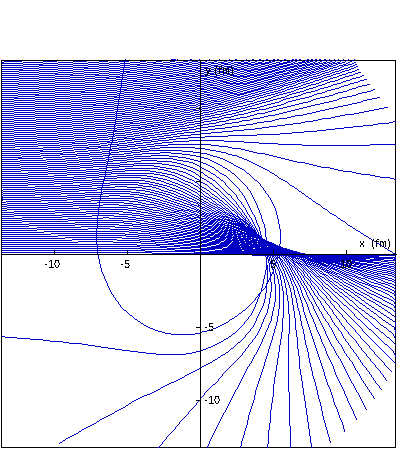
\includegraphics[width=.49\linewidth]{figures/010-clas-traj.png}
	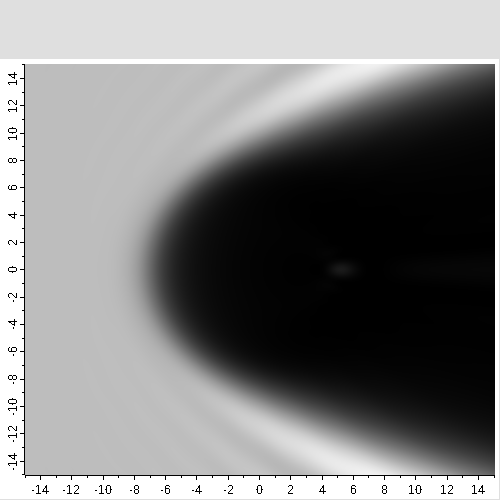
\includegraphics[width=.49\linewidth]{figures/010-omp3-bwpdf.png}
	\caption{Сравнение функции распределения и классических траекторий при энергии 30 МэВ.~\cite{26-28-30-34mev}}
	\label{fig:30mev-pdf-traj}
\end{figure}% }}}
\begin{figure}% abs, ratio, 30mev {{{
	\centering
	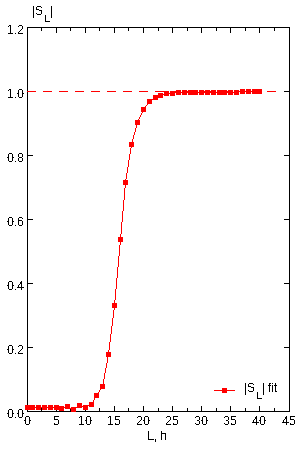
\includegraphics[width=.35\linewidth]{figures/010-omp3-s.png}
	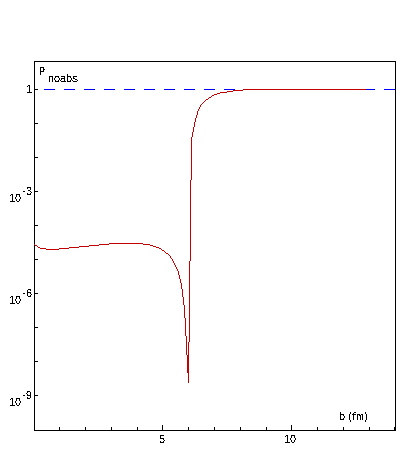
\includegraphics[width=.49\linewidth]{figures/010-clas-surv.png}
	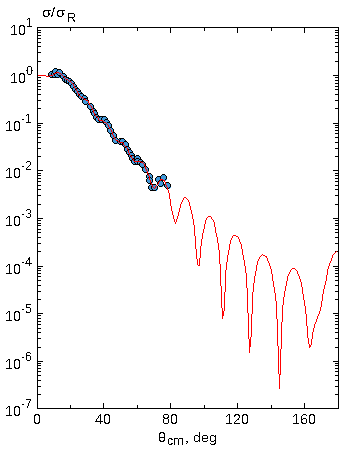
\includegraphics[width=.49\linewidth]{figures/010-omp3-ratio.png}
	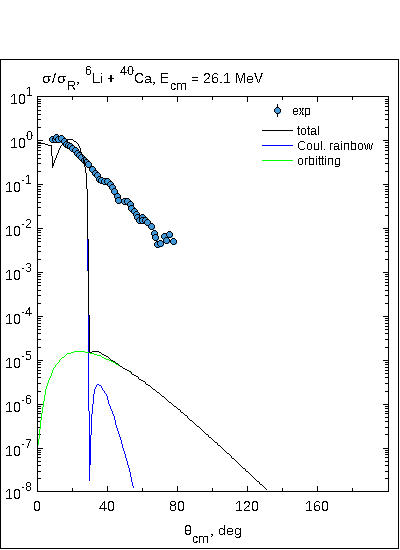
\includegraphics[width=.49\linewidth]{figures/010-clas-ratio.png}
	\caption{Сравнение квантовых и классических вероятностей поглощения и сечений при энергии 30 МэВ.~\cite{26-28-30-34mev}}
	\label{fig:30mev-abs-ratio}
\end{figure}% }}}

\begin{figure}% pdf, traj, 99mev {{{
	\centering
	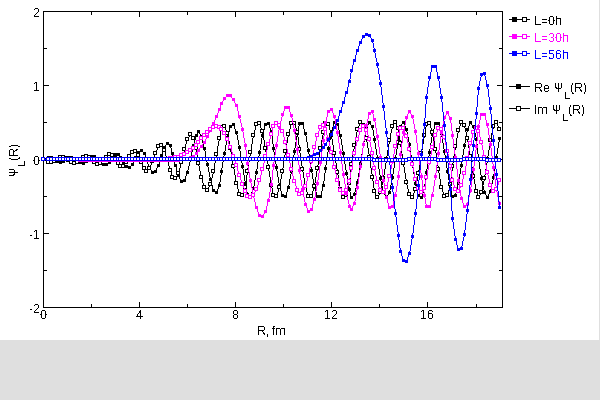
\includegraphics[width=.49\linewidth]{figures/014-omp1-psi.png}
	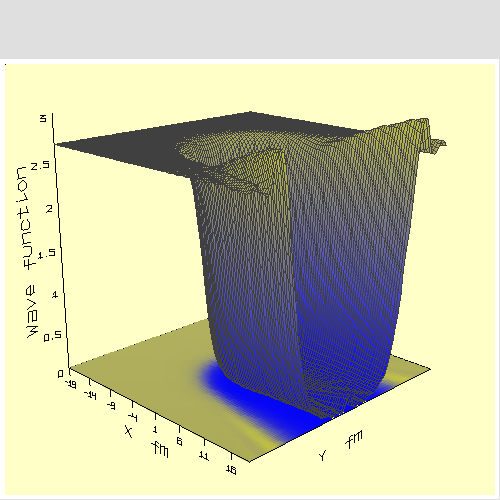
\includegraphics[width=.49\linewidth]{figures/014-omp1-pdf.png}
	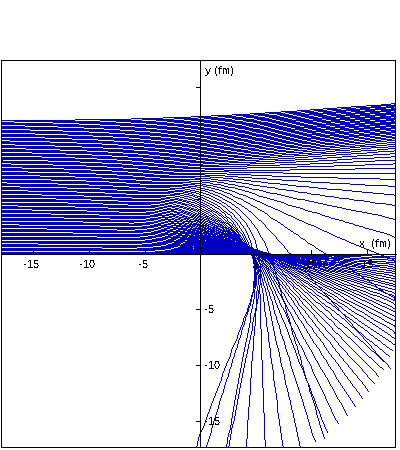
\includegraphics[width=.49\linewidth]{figures/014-clas-traj.png}
	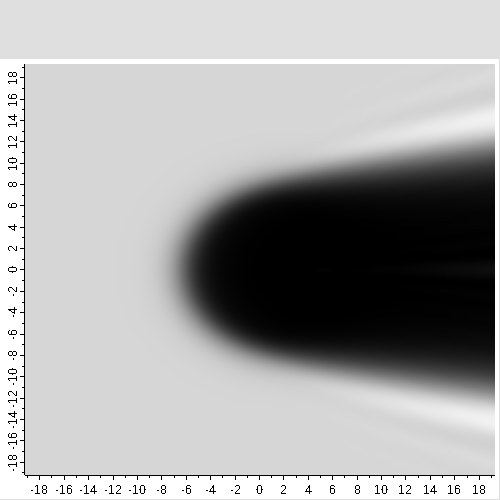
\includegraphics[width=.49\linewidth]{figures/014-omp1-bwpdf.png}
	\caption{Сравнение функции распределения и классических траекторий при энергии 99 МэВ.~\cite{99mev}}
	\label{fig:99mev-pdf-traj}
\end{figure}% }}}
\begin{figure}% abs, ratio, 99mev {{{
	\centering
	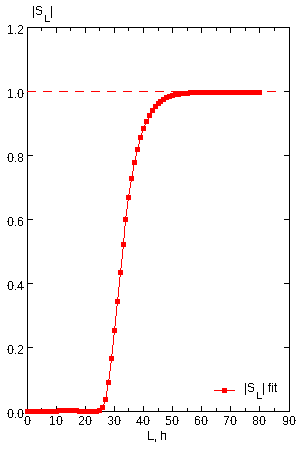
\includegraphics[width=.35\linewidth]{figures/014-omp1-s.png}
	\includegraphics[width=.49\linewidth]{figures/014-clas-surv.png}
	\includegraphics[width=.49\linewidth]{figures/014-omp1-ratio.png}
	\includegraphics[width=.49\linewidth]{figures/014-clas-ratio.png}
	\caption{Сравнение квантовых и классических вероятностей поглощения и сечений при энергии 99 МэВ.~\cite{99mev}}
	\label{fig:99mev-abs-ratio}
\end{figure}% }}}
% }}}

\clearpage
\begin{thebibliography}{99}% {{{
	\bibitem{20mev} K. Bethge, C. M. Fou, R. W. Zurm\"{u}hle, \textit{Elastic scattering of lithium nuclei}, \href{https://doi.org/10.1016/0375-9474(69)91001-X}{Nucl. Phys. A \textbf{123} (1969) 521--530}.

	\bibitem{26-28-30-34mev} J. Cook, K. W. Kemper, M. F. Vineyard, \textit{Description of large angle $^{6}\mathrm{Li}$ + $^{40}\mathrm{Ca}$ scattering from 26 to 34 MeV using double-folded and $\ensuremath{\alpha}+d$ cluster potentials}, \href{http://dx.doi.org/10.1103/PhysRevC.26.486}{Phys. Rev. C \textbf{26} (1982) 486--492}.

	\bibitem{28-34mev} R. I. Cutler, M. J. Nadworny, K. W. Kemper, \textit{28- and 34-MeV $^{6}\mathrm{Li}$ and $^{7}\mathrm{Li}$ elastic scattering on nuclei with $40\ensuremath{\le}A\ensuremath{\le}91$}, \href{https://dx.doi.org/10.1103/PhysRevC.15.1318}{Phys. Rev. C \textbf{15} (1977) 1318--1324}.

	\bibitem{30mev} H. Bohn \textit{et al.}, \textit{Back-angle anomalies in $^{6}\mathrm{Li}$ scattering from $^{40}\mathrm{Ca}$ and $^{44}\mathrm{Ca}$}, \href{http://dx.doi.org/10.1103/PhysRevC.16.665}{Phys. Rev. C \textbf{16} (1977) 665--672}.

	\bibitem{32mev} N. Anantaraman, H. W. Fulbright, P. M. Stwertka, \textit{Variation of ground-state $\ensuremath{\alpha}$\nobreakdash-particle strengths for $\mathrm{sd}$- and $\mathrm{fp}$-shell nuclei}, \href{http://dx.doi.org/10.1103/PhysRevC.22.501}{Phys. Rev. C \textbf{22} (1980) 501--506}.

	\bibitem{88mev} C. B. Fulmer \textit{et al.}, \textit{Elastic and inelastic scattering of 88 MeV $^6\mathrm{Li}$ ions}, \href{https://doi.org/10.1016/0375-9474(81)90125-1}{Nucl. Phys. A \textbf{356} (1981) 235--259}.

	\bibitem{99mev} P. Schwandt \textit{et al.}, \textit{Optical potential for $^{6}\mathrm{Li}$ elastic scattering at 99 MeV}, \href{http://dx.doi.org/10.1103/PhysRevC.24.1522}{Phys. Rev. C \textbf{24} (1981) 1522--1528}.

	\bibitem{156mev} J. Cook \textit{et al.}, \textit{Optical model studies of $^6\mathrm{Li}$ elastic scattering at 156 MeV}, \href{https://doi.org/10.1016/0375-9474(82)90514-0}{Nucl. Phys. A \textbf{388} (1982) 173--186}.

	\bibitem{210mev} A. Nadasen \textit{et al.}, \textit{Unique $^{6}\mathrm{nucleus}$ optical potentials from elastic scattering of 210 MeV $^{6}\mathrm{Li}$ ions by $^{28}\mathrm{Si}$, $^{40}\mathrm{Ca}$, $^{90}\mathrm{Zr}$, and $^{208}\mathrm{Pb}$}, \href{http://dx.doi.org/10.1103/PhysRevC.39.536}{Phys. Rev. C \textbf{39} (1989) 536--545}.

	\bibitem{240mev} Krishichayan \textit{et al.}, \textit{Elastic and inelastic scattering of 240-MeV $^{6}\mathrm{Li}$ ions from $^{40}\mathrm{Ca}$ and $^{48}\mathrm{Ca}$ and tests of a systematic optical potential}, \href{http://dx.doi.org/10.1103/PhysRevC.81.044612}{Phys. Rev. C \textbf{81} (2010) 044612}.

	\bibitem{nrv} \texttt{\href{http://nrv.jinr.ru/nrv/}{http://nrv.jinr.ru/nrv/}}

	\bibitem{tutorial} А. С. Деникин, М. А. Науменко, В. В. Самарин, \textit{Оптическая модель упругого рассеяния в базе знаний Nuclear Reaction Video (NRV)}, \href{http://nrv.jinr.ru/nrv/OM-Tutorial.pdf}{Дубна, 2016}.

	\bibitem{omp1} J. Cook, \textit{Global optical-model potentials for the elastic scattering of $^{6,\ 7}\mathrm{Li}$ projectiles}, \href{https://doi.org/10.1016/0375-9474(82)90513-9}{Nucl. Phys. A \textbf{388} (1982) 153--172}.

	\bibitem{omp2} R. Kalpakchieva, \textit{et al.} \textit{Elastic and inelastic scattering of $^{6}\mathrm{Li}$ on $^{12}\mathrm{C}$ at 63 MeV}, \href{http://www1.jinr.ru/Preprints/2003/132(P7-2003-132).pdf}{JINR Preprint \texttt{JINR-P7-2003-132}}.

	\bibitem{omp3} R. O. Akyuz and A. Winther, \textit{Parameterization of the nucleus-nucleus potential}, \href{http://nrv.jinr.ru/nrv/webnrv/elastic\_scattering/Akyuz.pdf}{Proc. Enrico Fermi Int. School of Physics, 1979, ``Nuclear structure and heavy-ion reactions'', ed. R. A. Broglia, C. H. Dasso and R. Ricci (North-Holland, Amsterdam, 1981) p. 491}.

\end{thebibliography}% }}}

\end{document}
